\documentclass[12pt,a4paper]{article}

% ── Encoding ──────────────────────────────────────────────────────────────────
\usepackage[T1]{fontenc}        % correct rendering of < > in \texttt{}
\usepackage[utf8]{inputenc}     % UTF-8 source encoding

% ── Packages ──────────────────────────────────────────────────────────────────
\usepackage[margin=1in]{geometry}
\usepackage{amsmath,amssymb}
\usepackage{booktabs}
\usepackage{graphicx}
\usepackage{xcolor}
\usepackage{caption}
\usepackage{subcaption}
\usepackage{multirow}
\usepackage{array}
\usepackage{enumitem}
\usepackage{titlesec}
\usepackage{parskip}
\usepackage{microtype}
\usepackage{listings}
\usepackage{float}
\usepackage{cite}
\usepackage{hyperref}           % must be loaded LAST among packages

% ── Image paths (upload PNG files to Overleaf preserving directory structure) ─
% Directory layout expected on Overleaf:
%   part1nmt/outputs/random/   — loss_plot.png, bleu_plot.png, chrf_plot.png, lr_plot.png
%   part1nmt/outputs/bert/     — loss_plot.png, bleu_plot.png, chrf_plot.png, lr_plot.png
%   part1nmt/outputs/comparison/ — bleu_comparison_test.png, chrf_comparison_test.png
%   part2/outputs/bert_pretrain/ — loss_plot.png, val_ppl_plot.png, train_ppl_plot.png, lr_plot.png
%   part2/outputs/gpt_pretrain/  — loss_plot.png, val_ppl_plot.png, train_ppl_plot.png, lr_plot.png
%   part2/outputs/translation/   — loss_plot.png, bleu_plot.png, chrf_plot.png, lr_plot.png

\hypersetup{
    colorlinks=true,
    linkcolor=blue!60!black,
    citecolor=blue!60!black,
    urlcolor=blue!60!black
}

\lstset{
    basicstyle=\small\ttfamily,
    backgroundcolor=\color{gray!10},
    frame=single,
    breaklines=true,
    captionpos=b
}

% ── Title ─────────────────────────────────────────────────────────────────────
\title{
    \vspace{-1cm}
    \Large\textbf{Hindi $\leftrightarrow$ Marathi Neural Machine Translation} \\[0.4em]
    \large Technical Report — AdiVaani Hiring Assessment \\[0.2em]
    \normalsize MISN Lab, IIT Delhi
}
\author{
    Rajnish Maurya \\[0.3em]
    \small\texttt{mauryarajnish73@gmail.com} \\[0.2em]
    \small\href{https://github.com/Rajnishmaurya/MISN-LAB-Assignment}{\texttt{github.com/Rajnishmaurya/MISN-LAB-Assignment}}
}
\date{May 25, 2026}

% ══════════════════════════════════════════════════════════════════════════════
\begin{document}
\maketitle
\tableofcontents
\newpage

% ══════════════════════════════════════════════════════════════════════════════
\section{Abstract}

This report presents a two-part study on Hindi$\leftrightarrow$Marathi Neural Machine Translation (NMT).
\textbf{Part 1} implements a classical Seq2Seq architecture with LSTM encoder-decoder and Bahdanau additive attention, comparing two embedding strategies: randomly initialized embeddings versus embeddings pre-initialized from BERT models trained on Hindi and Marathi text.
\textbf{Part 2} pretrains a BERT-like bidirectional encoder ($\sim$100M parameters) and a GPT-2 style autoregressive decoder ($\sim$125M parameters) entirely from scratch on monolingual Hindi and Marathi text, then combines them into an encoder-decoder translation model via cross-attention fine-tuning.
All Part 2 architectures implement three required modifications: Rotary Positional Embeddings (RoPE), Grouped Query Attention (GQA), and RMSNorm.
The pretrained encoder-decoder system achieves BLEU(100) = 25.46 and CHRF++(100) = 57.71 on the test set — a significant improvement over the classical LSTM model (BLEU = 2.00, CHRF++ = 9.34 with beam search).

% ══════════════════════════════════════════════════════════════════════════════
\section{Introduction}

Hindi and Marathi are two closely related Indo-Aryan languages sharing the Devanagari script, overlapping vocabulary, and similar syntactic structures. Despite this proximity, automatic translation between them remains a non-trivial task due to morphological richness, dialectal variation, and limited parallel corpora relative to high-resource language pairs.

This assignment explores two paradigms of NMT:

\begin{enumerate}
    \item \textbf{Classical recurrent architectures}: Seq2Seq with LSTM encoder-decoder and attention, a well-understood baseline with interpretable components.
    \item \textbf{Modern Transformer-based pretraining}: Dedicated language model pretraining followed by fine-tuning, reflecting state-of-the-art practice.
\end{enumerate}

The bidirectional nature of the task (Hindi$\to$Marathi and Marathi$\to$Hindi simultaneously) is handled in both parts using direction tokens, allowing a single model to perform both translation directions.

% ══════════════════════════════════════════════════════════════════════════════
\section{Dataset and Preprocessing}

\subsection{Dataset}

A Hindi–Marathi parallel corpus was provided for this assignment. The raw data consists of aligned sentence pairs in Hindi (\texttt{.hi}) and Marathi (\texttt{.mr}) files. Table~\ref{tab:dataset} summarizes the data splits.

\begin{table}[H]
\centering
\caption{Dataset splits (bidirectional; each pair appears twice)}
\label{tab:dataset}
\begin{tabular}{lccc}
\toprule
\textbf{Split} & \textbf{Original Pairs} & \textbf{Bidirectional Pairs} & \textbf{Source} \\
\midrule
Train  & $\sim$217,500 & $\sim$435,000 & Assignment dataset \\
Valid  & $\sim$24,200  & $\sim$48,400  & 10\% split from train \\
Test   & $\sim$10,390  & $\sim$20,780  & Assignment dataset \\
\bottomrule
\end{tabular}
\end{table}

\subsection{Validation Split}

The original training set is split 90\%/10\% (seed = 42) to create the validation set. The test set is held out and used only for final evaluation.

\subsection{Bidirectional Data Augmentation}

Each original sentence pair is converted into two training examples using direction tokens prepended to the source:

\begin{itemize}
    \item \texttt{<hi2mr>} $\langle$Hindi source$\rangle$ $\to$ $\langle$Marathi target$\rangle$
    \item \texttt{<mr2hi>} $\langle$Marathi source$\rangle$ $\to$ $\langle$Hindi target$\rangle$
\end{itemize}

This effectively doubles the training data and trains a single unified model for both directions. At inference, the appropriate direction token is prepended to steer generation.

% ══════════════════════════════════════════════════════════════════════════════
\section{Tokenization}

\subsection{Part 1 Tokenizer}

A shared SentencePiece Byte Pair Encoding (BPE) tokenizer is trained on the combined source and target training corpus:

\begin{lstlisting}[language=bash, caption={Tokenizer training for Part 1}]
cat data/train.src data/train.tgt > final_combined.txt
python create_tokenizer.py  # trains spm.model
\end{lstlisting}

\begin{table}[H]
\centering
\caption{Part 1 tokenizer special tokens}
\begin{tabular}{lc}
\toprule
\textbf{Token} & \textbf{ID} \\
\midrule
PAD & 0 \\
BOS \texttt{<s>} & 1 \\
EOS \texttt{</s>} & 2 \\
UNK & 3 \\
\bottomrule
\end{tabular}
\end{table}

\textbf{Design rationale:} A single shared vocabulary for both Hindi and Marathi exploits the large subword overlap between the two Devanagari-script languages, improving generalization for rare words. Vocabulary size of 16,000 BPE tokens is sufficient to cover the full Unicode Devanagari range.

\subsection{Part 2 Tokenizer}

Part 2 uses a \emph{separate} tokenizer because BERT pretraining with Masked Language Modeling (MLM) requires a dedicated \texttt{[MASK]} token. The Part 1 tokenizer does not include this token.

\begin{table}[H]
\centering
\caption{Part 2 tokenizer special tokens}
\begin{tabular}{lc}
\toprule
\textbf{Token} & \textbf{ID} \\
\midrule
PAD & 0 \\
BOS \texttt{<s>} & 1 \\
EOS \texttt{</s>} & 2 \\
UNK & 3 \\
\textbf{[MASK]} & \textbf{4} \\
\bottomrule
\end{tabular}
\end{table}

The \texttt{[MASK]} token is registered via \texttt{user\_defined\_symbols=['[MASK]']} in SentencePiece, which assigns it ID=4 before any learned BPE pieces. Vocabulary size is kept at 16,000 for embedding compatibility across experiments.

% ══════════════════════════════════════════════════════════════════════════════
\section{Part 1 — Classical Neural Machine Translation}

\subsection{Architecture Overview}

The system implements a standard Seq2Seq architecture with the following components:

\subsubsection{Encoder}

A 2-layer bidirectional LSTM processes the source token sequence:

\[
\overrightarrow{h_t}, \overleftarrow{h_t} = \text{BiLSTM}(e_t, h_{t-1})
\]
\[
h_t = [\overrightarrow{h_t};\overleftarrow{h_t}] \in \mathbb{R}^{2d}
\]

where $e_t$ is the token embedding and $d = 512$ is the hidden dimension per direction.

\subsubsection{Bahdanau Attention}

Additive attention computes a context vector at each decoder step $i$:

\[
e_{ij} = \mathbf{v}^\top \tanh(\mathbf{W}_1 s_i + \mathbf{W}_2 h_j)
\]
\[
\alpha_{ij} = \text{softmax}(e_{ij})
\]
\[
c_i = \sum_j \alpha_{ij} \cdot h_j
\]

where $s_i$ is the decoder hidden state and $h_j$ are encoder output states.
An important optimization: $\mathbf{W}_2 h_j$ is precomputed once per batch before the decoding loop, avoiding redundant matrix multiplications at every decoder step.

\subsubsection{Decoder}

A 2-layer LSTM decoder receives the concatenation of the current token embedding and the context vector:

\[
s_i = \text{LSTM}([e_{y_{i-1}}; c_i], s_{i-1})
\]
\[
P(y_i | y_{<i}, X) = \text{softmax}(\mathbf{W}_o s_i)
\]

\textbf{Teacher forcing}: During training, ground-truth tokens are fed with probability 0.5; the model's own predictions are used for the remaining 0.5. During evaluation, teacher forcing is set to 0.0 for honest autoregressive generation.

\subsection{Embedding Strategies}

\subsubsection{Experiment 1: Random Initialization}

Embeddings of dimension 256 are initialized from $\mathcal{U}(-0.1, 0.1)$ and updated end-to-end during training. Total model parameters: \textbf{25.3M}.

\subsubsection{Experiment 2: BERT Pre-initialization}

Embeddings of dimension 768 are initialized from pretrained BERT models:
\begin{itemize}
    \item Encoder embeddings: \texttt{l3cube-pune/hindi-bert-v2}
    \item Decoder embeddings: \texttt{l3cube-pune/marathi-bert-v2}
\end{itemize}

Since the BERT models use WordPiece tokenization while our model uses SentencePiece BPE, a vocabulary alignment procedure is required. For each SentencePiece BPE token, the procedure:
\begin{enumerate}
    \item Tokenizes the BPE piece using the BERT WordPiece tokenizer
    \item Retrieves the BERT embedding vectors for the resulting sub-pieces
    \item Averages those vectors to obtain the initialization for the SentencePiece token
\end{enumerate}

These embeddings are fully trainable — they are initialized from BERT but updated throughout training. Total model parameters: \textbf{43.8M}.

\subsection{Beam Search Decoding}

Beam search with width $k=2$ is used for final evaluation. The score of a hypothesis $y$ of length $|y|$ is normalized by a length penalty to prevent the decoder from preferring shorter sequences:

\[
\text{score}(y) = \frac{\log P(y|X)}{|y|^{0.6}}
\]

\subsection{Hyperparameters}

\begin{table}[H]
\centering\small
\caption{Part 1 hyperparameters}
\label{tab:part1_hparams}
\begin{tabular}{lcc}
\toprule
\textbf{Parameter} & \textbf{Random} & \textbf{BERT} \\
\midrule
Embedding dim & 256 & 768 \\
Hidden dim (LSTM) & 512 & 512 \\
LSTM layers & 2 & 2 \\
Dropout & 0.3 & 0.3 \\
Vocab size & 16,000 & 16,000 \\
Max sequence length & 128 & 128 \\
Batch size & 256 & 128 \\
Optimizer & AdamW & AdamW \\
Weight decay & $10^{-2}$ & $10^{-2}$ \\
Learning rate & $10^{-4}$ & $10^{-4}$ \\
Minimum LR & $10^{-6}$ & $10^{-6}$ \\
LR schedule & 2-epoch warmup + cosine decay & Same \\
Label smoothing & 0.1 & 0.1 \\
Gradient clipping & 1.0 (norm) & 1.0 (norm) \\
Epochs & 10 & 10 \\
Teacher forcing ratio & 0.5 (train) / 0.0 (eval) & Same \\
\bottomrule
\end{tabular}
\end{table}

\subsection{Training Results}

\subsubsection{Random Embeddings — Per-Epoch Metrics}

\begin{table}[H]
\centering
\caption{Random embeddings: per-epoch training and validation metrics}
\label{tab:random_epochs}
\resizebox{\textwidth}{!}{%
\begin{tabular}{ccccccc}
\toprule
\textbf{Epoch} & \textbf{Train Loss} & \textbf{Val Loss} & \textbf{Train BLEU} & \textbf{Val BLEU} & \textbf{Train CHRF++} & \textbf{Val CHRF++} \\
\midrule
1  & 8.349 & 7.726 & 0.00 & 0.00 & 9.01  & 0.67  \\
2  & 7.648 & 7.256 & 0.02 & 0.06 & 0.67  & 4.17  \\
3  & 7.206 & 6.996 & 0.08 & 0.38 & 4.59  & 5.89  \\
4  & 6.985 & 6.907 & 0.22 & 0.48 & 6.60  & 6.30  \\
5  & 6.850 & 6.838 & 0.26 & 0.75 & 7.87  & 6.66  \\
6  & 6.755 & 6.796 & 0.36 & 1.03 & 8.52  & 7.57  \\
7  & 6.687 & 6.767 & 0.43 & 1.18 & 9.74  & 7.72  \\
8  & 6.654 & 6.752 & 0.49 & 1.34 & 10.21 & 8.15  \\
\textbf{9*} & \textbf{6.627} & \textbf{6.736} & \textbf{0.50} & \textbf{1.23} & \textbf{10.45} & \textbf{7.98}  \\
10 & 6.616 & 6.737 & 0.47 & 1.28 & 10.78 & 8.07  \\
\bottomrule
\end{tabular}%
}
\par\smallskip\noindent{\small * Best checkpoint (lowest validation loss)}
\end{table}

\begin{figure}[H]
\centering
\begin{subfigure}[b]{0.48\textwidth}
    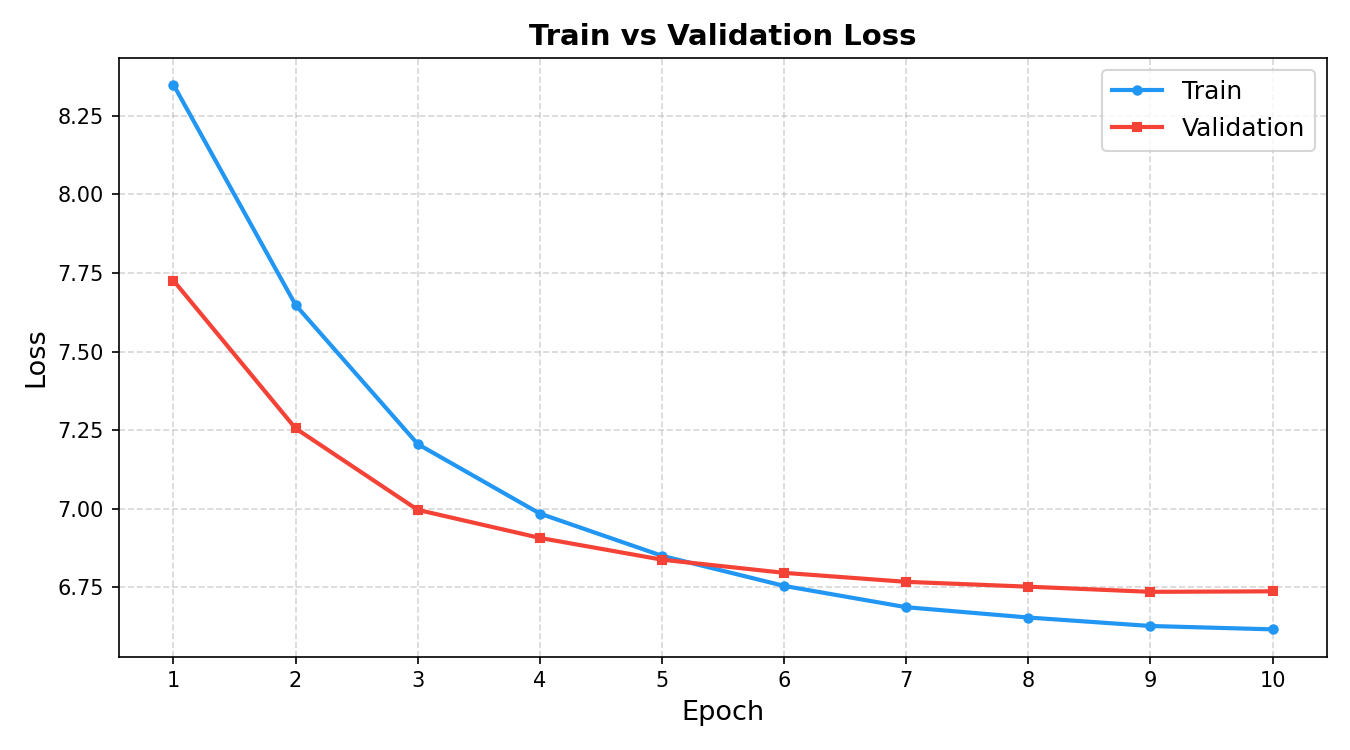
\includegraphics[width=\textwidth]{part1nmt/outputs/random/loss_plot.png}
    \caption{Train and validation loss}
\end{subfigure}
\hfill
\begin{subfigure}[b]{0.48\textwidth}
    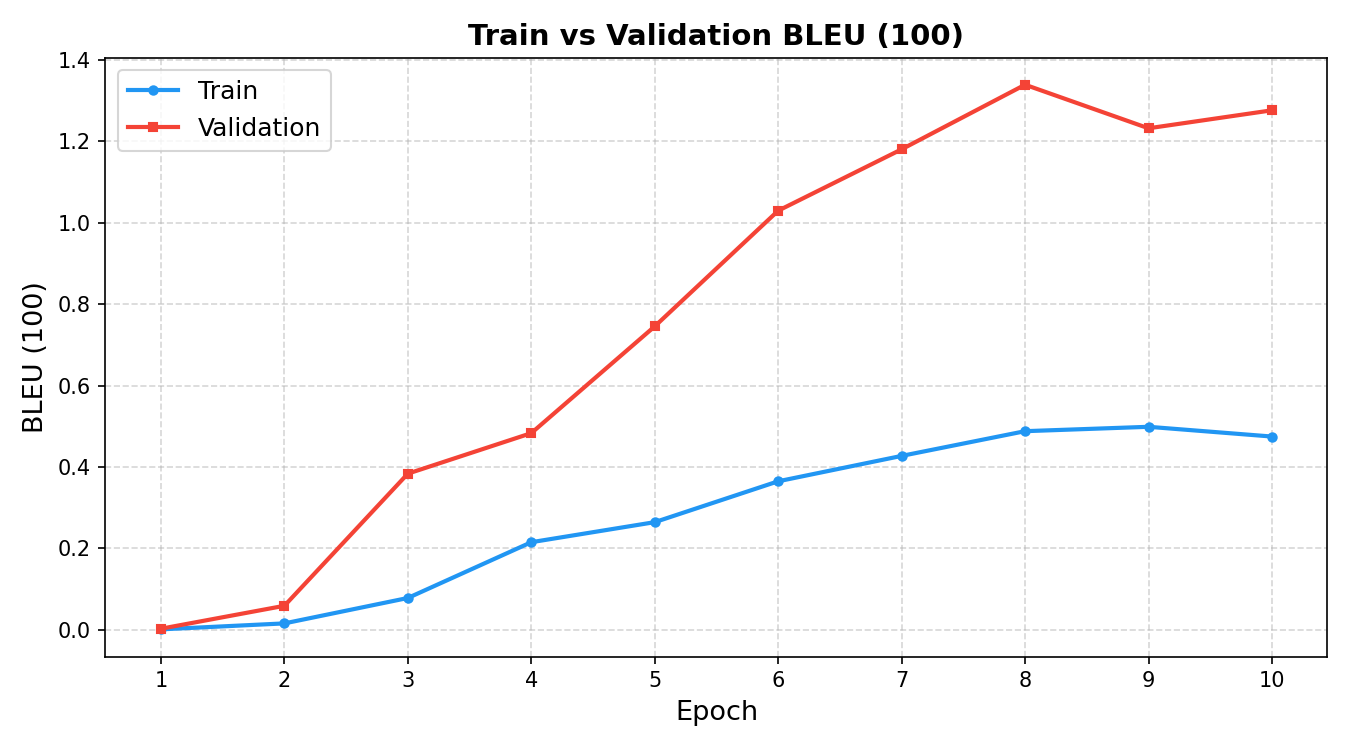
\includegraphics[width=\textwidth]{part1nmt/outputs/random/bleu_plot.png}
    \caption{Train and validation BLEU}
\end{subfigure}

\vspace{0.5em}

\begin{subfigure}[b]{0.48\textwidth}
    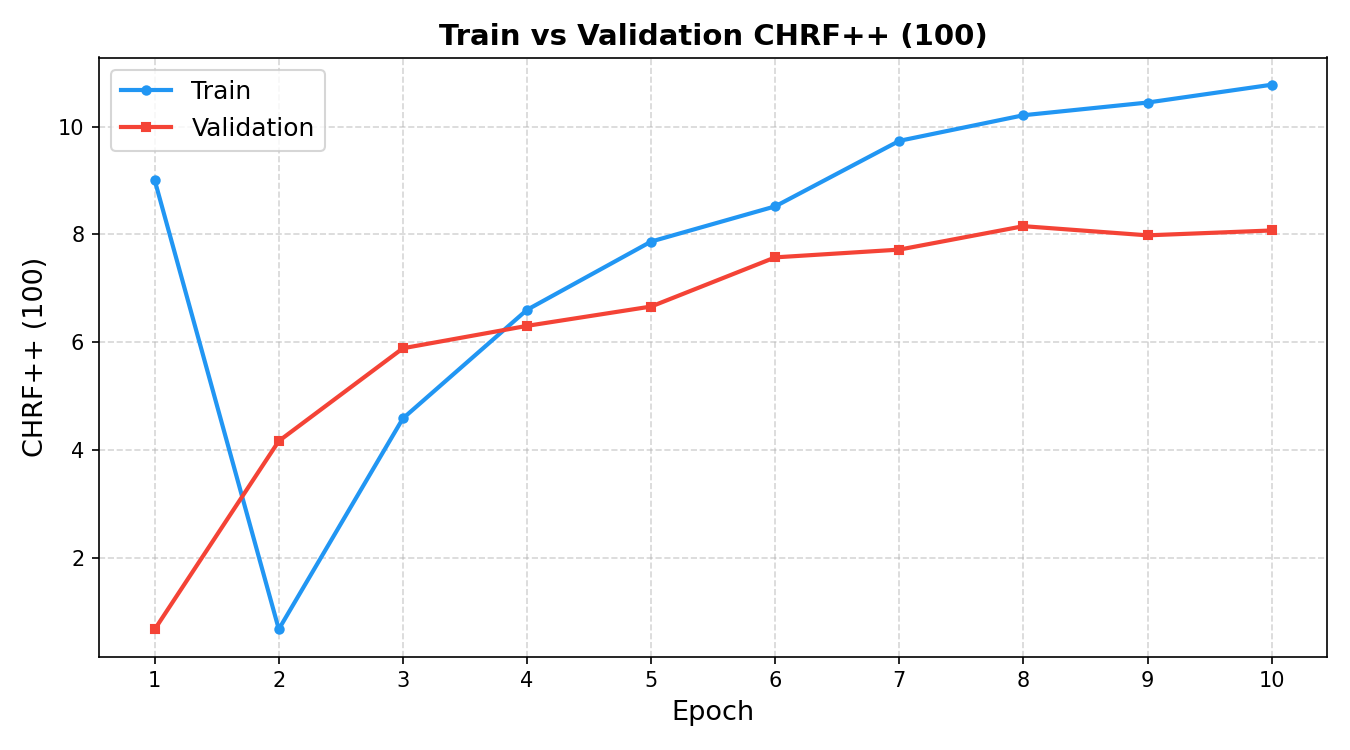
\includegraphics[width=\textwidth]{part1nmt/outputs/random/chrf_plot.png}
    \caption{Train and validation CHRF++}
\end{subfigure}
\hfill
\begin{subfigure}[b]{0.48\textwidth}
    \includegraphics[width=\textwidth]{part1nmt/outputs/random/lr_plot.png}
    \caption{Learning rate schedule}
\end{subfigure}
\caption{Part 1 — Random Embeddings: training curves over 10 epochs.}
\label{fig:random_training}
\end{figure}

\subsubsection{BERT Embeddings — Per-Epoch Metrics}

\begin{table}[H]
\centering
\caption{BERT embeddings: per-epoch training and validation metrics}
\label{tab:bert_epochs}
\resizebox{\textwidth}{!}{%
\begin{tabular}{ccccccc}
\toprule
\textbf{Epoch} & \textbf{Train Loss} & \textbf{Val Loss} & \textbf{Train BLEU} & \textbf{Val BLEU} & \textbf{Train CHRF++} & \textbf{Val CHRF++} \\
\midrule
1  & 8.229 & 7.660 & 0.00 & 0.00 & 3.79  & 1.12  \\
2  & 7.585 & 7.158 & 0.02 & 0.05 & 1.10  & 3.78  \\
3  & 7.065 & 6.976 & 0.03 & 0.24 & 4.70  & 4.63  \\
4  & 6.790 & 6.874 & 0.22 & 0.66 & 8.16  & 6.54  \\
5  & 6.643 & 6.819 & 0.34 & 0.57 & 9.82  & 6.42  \\
6  & 6.547 & 6.774 & 0.48 & 0.68 & 10.42 & 7.16  \\
7  & 6.483 & 6.741 & 0.49 & 0.80 & 10.83 & 7.40  \\
8  & 6.437 & 6.711 & 0.50 & 0.78 & 11.16 & 7.55  \\
9  & 6.414 & 6.707 & 0.60 & 0.79 & 11.27 & 7.61  \\
\textbf{10*}& \textbf{6.406} & \textbf{6.703} & \textbf{0.52} & \textbf{0.80} & \textbf{11.10} & \textbf{7.68} \\
\bottomrule
\end{tabular}%
}
\par\smallskip\noindent{\small * Best checkpoint (lowest validation loss)}
\end{table}

\begin{figure}[H]
\centering
\begin{subfigure}[b]{0.48\textwidth}
    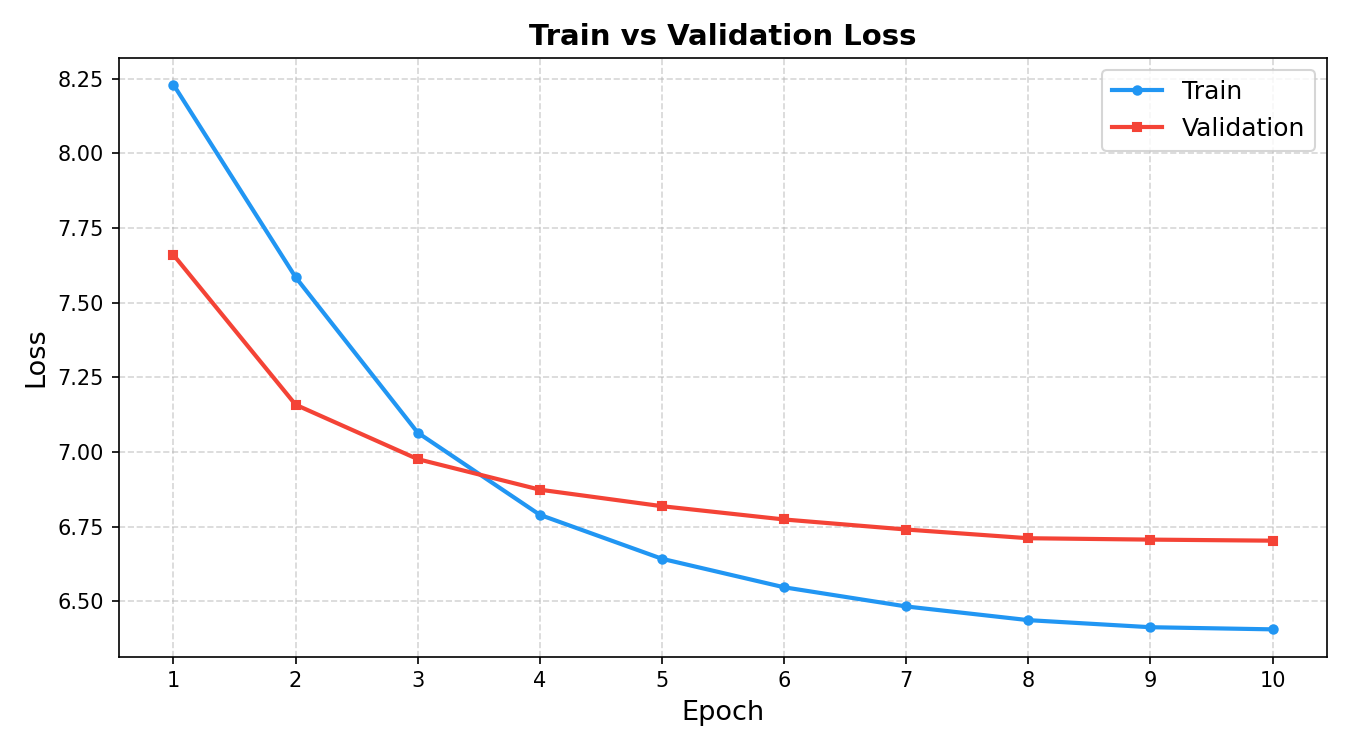
\includegraphics[width=\textwidth]{part1nmt/outputs/bert/loss_plot.png}
    \caption{Train and validation loss}
\end{subfigure}
\hfill
\begin{subfigure}[b]{0.48\textwidth}
    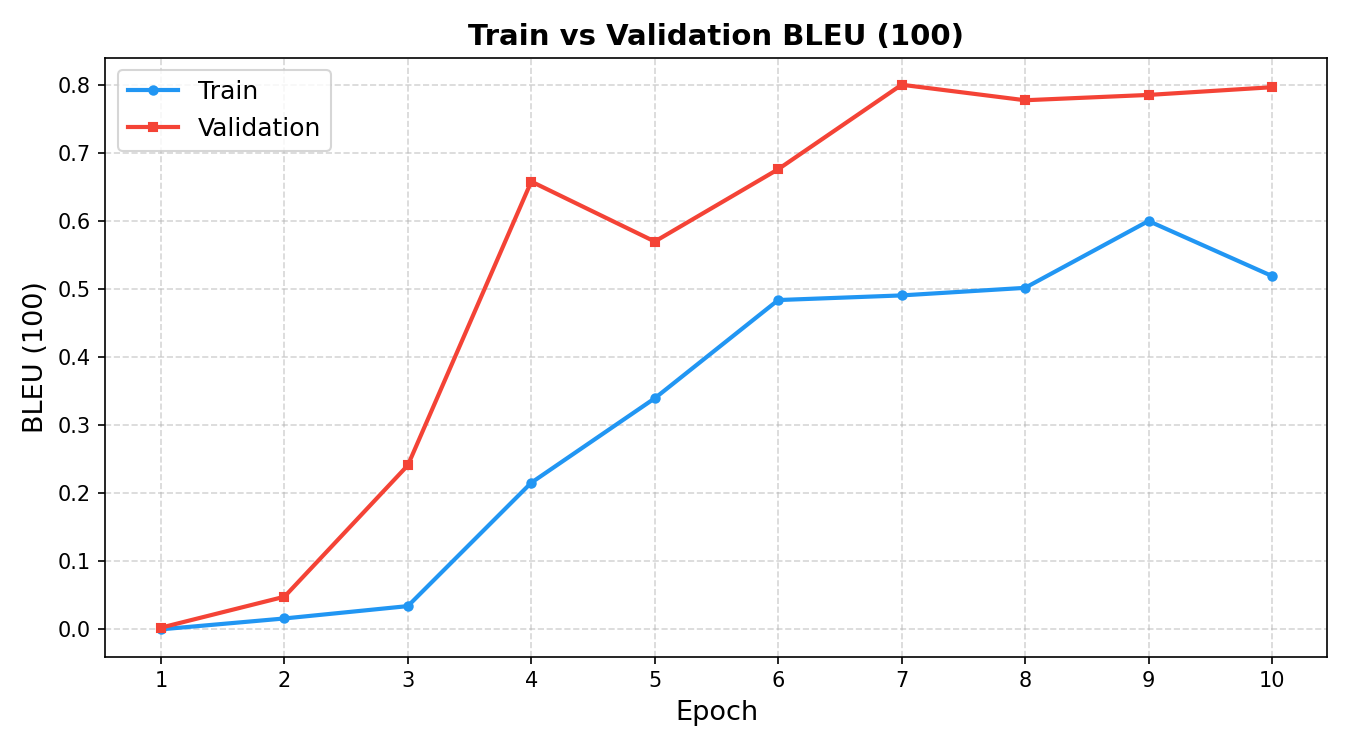
\includegraphics[width=\textwidth]{part1nmt/outputs/bert/bleu_plot.png}
    \caption{Train and validation BLEU}
\end{subfigure}

\vspace{0.5em}

\begin{subfigure}[b]{0.48\textwidth}
    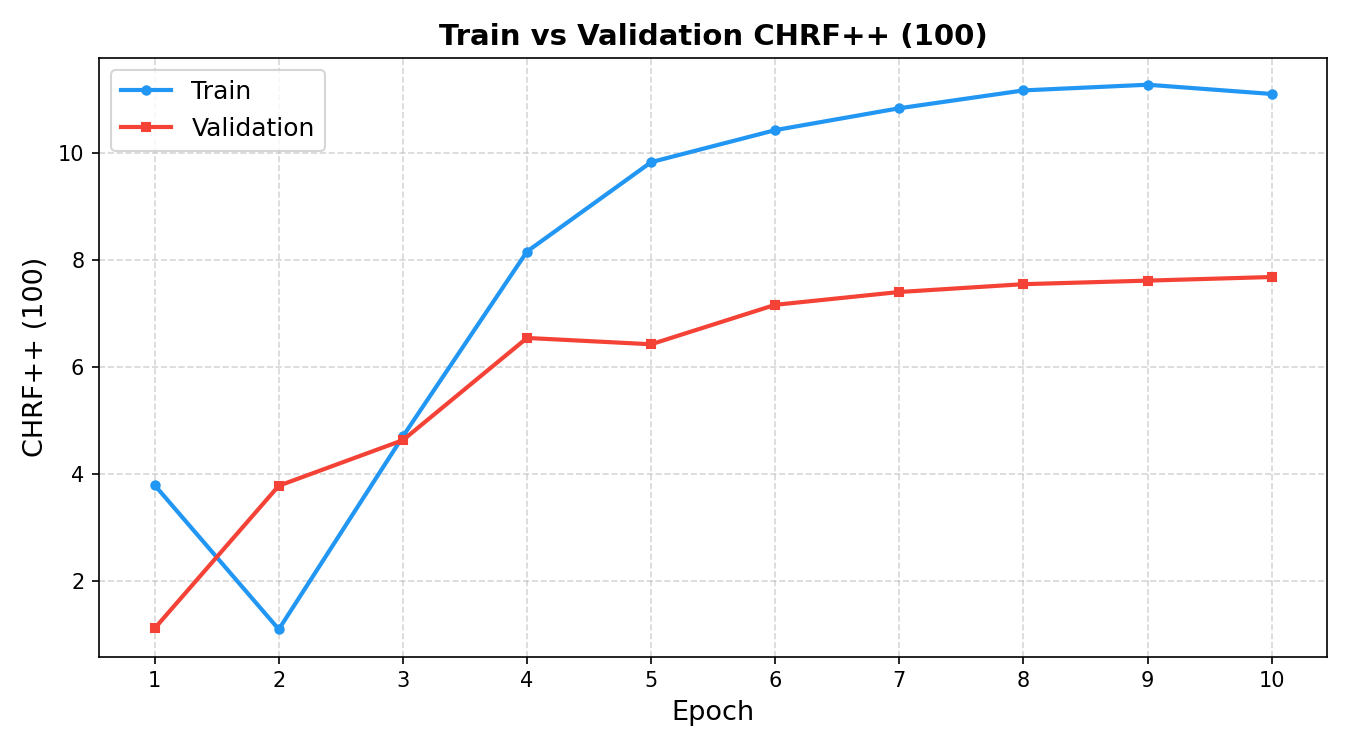
\includegraphics[width=\textwidth]{part1nmt/outputs/bert/chrf_plot.png}
    \caption{Train and validation CHRF++}
\end{subfigure}
\hfill
\begin{subfigure}[b]{0.48\textwidth}
    \includegraphics[width=\textwidth]{part1nmt/outputs/bert/lr_plot.png}
    \caption{Learning rate schedule}
\end{subfigure}
\caption{Part 1 — BERT Embeddings: training curves over 10 epochs.}
\label{fig:bert_training}
\end{figure}

\subsection{Final Test Results}

\begin{table}[H]
\centering\small
\caption{Part 1 test set results (20,780 examples)}
\label{tab:part1_results}
\begin{tabular}{lcccc}
\toprule
\textbf{Model} & \textbf{Test Loss} & \textbf{BLEU (100)} & \textbf{CHRF++ (100)} & \textbf{Training Time} \\
\midrule
Random embeddings (greedy) & 6.790 & 1.66 & 8.47 & 7.40 h \\
BERT embeddings (greedy)   & 6.752 & 0.97 & 7.96 & 7.31 h \\
\midrule
Random embeddings (beam=2) & — & 2.00 & 9.34 & — \\
BERT embeddings (beam=2)   & — & 1.98 & 9.46 & — \\
\bottomrule
\end{tabular}
\end{table}

\begin{figure}[H]
\centering
\begin{subfigure}[b]{0.48\textwidth}
    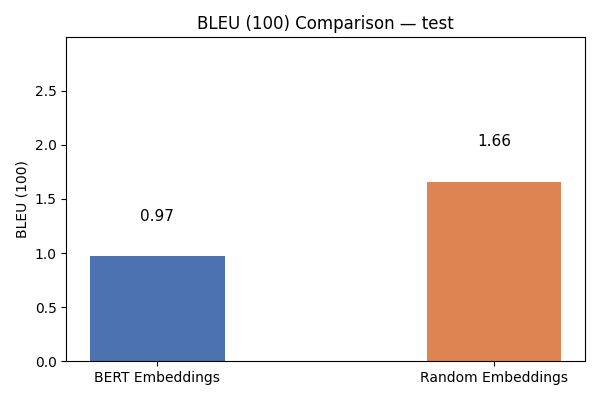
\includegraphics[width=\textwidth]{part1nmt/outputs/comparison/bleu_comparison_test.png}
    \caption{BLEU comparison (test set)}
\end{subfigure}
\hfill
\begin{subfigure}[b]{0.48\textwidth}
    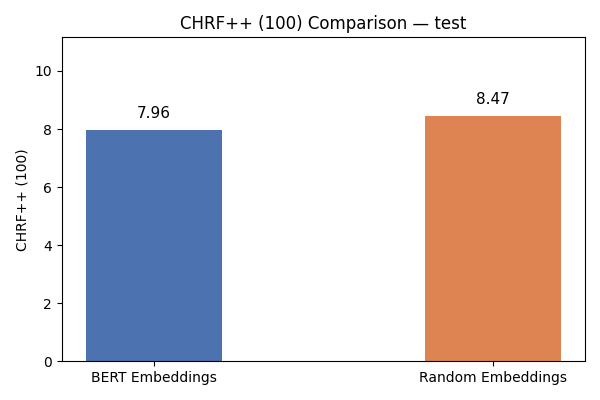
\includegraphics[width=\textwidth]{part1nmt/outputs/comparison/chrf_comparison_test.png}
    \caption{CHRF++ comparison (test set)}
\end{subfigure}
\caption{Part 1 — Test set comparison between Random and BERT embedding models under greedy and beam search decoding.}
\label{fig:part1_comparison}
\end{figure}

\subsection{Analysis}

\subsubsection{Why are scores low?}

The absolute BLEU and CHRF++ scores are low for several reasons:
\begin{enumerate}
    \item \textbf{Limited epochs}: Only 10 training epochs were run. LSTM-based NMT systems typically require 20–50 epochs on larger datasets to converge fully.
    \item \textbf{Model capacity}: The hidden dimension of 512 and 2 LSTM layers represent a relatively small model for the task.
    \item \textbf{Translation difficulty}: Hindi$\leftrightarrow$Marathi involves morphological agglutination, free word order, and script-identical but semantically distinct tokens.
\end{enumerate}

\subsubsection{Random vs. BERT Embeddings}

Counterintuitively, the random embedding model slightly outperforms the BERT-initialized model on BLEU (1.66 vs 0.97 greedy). Several factors explain this:

\begin{enumerate}
    \item \textbf{Vocabulary mismatch}: The BERT models use WordPiece tokenization; mapping them to SentencePiece BPE tokens via vector averaging is an approximation that introduces noise, especially for BPE pieces that do not map cleanly to WordPiece sub-units.
    \item \textbf{Dimensionality}: The random model uses 256-dimensional embeddings matched to the 512-dimensional LSTM, while the BERT model uses 768-dimensional embeddings passed into the same 512-dimensional LSTM — the larger projection may not be fully utilized in 10 epochs.
    \item \textbf{Training instability}: BERT embeddings carry language-specific priors that may conflict with the shared-vocabulary bilingual setup, causing slower or suboptimal optimization.
\end{enumerate}

However, in beam search evaluation the gap narrows (BERT achieves slightly better CHRF++: 9.46 vs 9.34), suggesting BERT embeddings may produce more linguistically coherent outputs even at lower BLEU.

\subsubsection{Training Dynamics}

Both models show the expected pattern: rapid loss decrease in early epochs (1–5) followed by slower improvement (Figures~\ref{fig:random_training} and~\ref{fig:bert_training}). Training BLEU continues to improve past epoch 6 while validation BLEU plateaus, indicating mild overfitting. Beam search consistently outperforms greedy decoding on both BLEU and CHRF++, confirming the benefit of the length penalty (Figure~\ref{fig:part1_comparison}).

% ══════════════════════════════════════════════════════════════════════════════
\section{Part 2 — Language Model Pretraining and Translation}

\subsection{Architectural Modifications}

All three required architectural modifications are implemented from scratch. Table~\ref{tab:arch_mods} summarizes the changes.

\begin{table}[H]
\centering
\caption{Architectural modifications from standard Transformer}
\label{tab:arch_mods}
\begin{tabular}{lll}
\toprule
\textbf{Component} & \textbf{Standard} & \textbf{This Implementation} \\
\midrule
Positional Embeddings & Sinusoidal / Learned & \textbf{RoPE} \cite{su2021roformer} \\
Attention & Multi-Head Attention & \textbf{GQA} \cite{ainslie2023gqa} \\
Normalization & LayerNorm & \textbf{RMSNorm} \cite{zhang2019rmsnorm} \\
\bottomrule
\end{tabular}
\end{table}

\subsubsection{Rotary Positional Embeddings (RoPE)}

RoPE encodes positional information by rotating query and key vectors in complex space. For a query/key vector $\mathbf{x}$ at position $t$ and head dimension $d_h$:

\[
\text{RoPE}(\mathbf{x}, t)_j = \begin{cases}
x_j \cos(t\theta_j) - x_{j+1}\sin(t\theta_j) & j \text{ even} \\
x_{j-1}\sin(t\theta_{j-1}) + x_j\cos(t\theta_{j-1}) & j \text{ odd}
\end{cases}
\]

where $\theta_j = 10000^{-2j/d_h}$.

Key properties:
\begin{itemize}
    \item No learned positional embedding table
    \item The dot product $\langle\text{RoPE}(\mathbf{q}, m), \text{RoPE}(\mathbf{k}, n)\rangle$ depends only on $m-n$, encoding relative position
    \item Applied only to self-attention query and key vectors; \textbf{not applied in cross-attention}
\end{itemize}

\subsubsection{Root Mean Square Normalization (RMSNorm)}

RMSNorm normalizes only by the root mean square, removing the mean subtraction and bias of LayerNorm:

\[
\text{RMSNorm}(\mathbf{x}) = \frac{\mathbf{x}}{\text{RMS}(\mathbf{x})} \cdot \mathbf{w}, \quad \text{RMS}(\mathbf{x}) = \sqrt{\frac{1}{d}\sum_{i=1}^d x_i^2 + \varepsilon}
\]

The normalization is computed in \texttt{float32} for numerical stability, with the result cast back to the input dtype. The only learnable parameter is $\mathbf{w} \in \mathbb{R}^d$ (no bias).

\subsubsection{Grouped Query Attention (GQA)}

GQA reduces the number of key-value (KV) heads while keeping the number of query heads fixed:

\[
\text{num\_heads} = 12,\quad \text{num\_kv\_heads} = 4,\quad \text{groups} = 3
\]

Each KV head is shared by 3 query heads, reducing KV projection parameters by $3\times$. The KV expansion in practice uses:

\begin{lstlisting}[language=python, caption={KV expansion in GQA}]
k = k.repeat_interleave(groups, dim=1)   # (B, 12, T, d_h)
v = v.repeat_interleave(groups, dim=1)   # (B, 12, T, d_h)
\end{lstlisting}

In cross-attention, RoPE is skipped (\texttt{is\_cross\_attn=True}) since the encoder and decoder sequences have independent position indices that should not be mixed via RoPE rotations.

\subsection{BERT-like Encoder}

\begin{lstlisting}[caption={BERT encoder architecture}]
Token Embedding (vocab=16000, dim=768)
    |
12 x EncoderLayer:
    RMSNorm -> GQA Self-Attention (bidirectional, RoPE) -> Residual
    RMSNorm -> FFN (Linear -> GELU -> Linear) -> Residual
    |
RMSNorm (final)
    |
MLM Head: Linear(768 -> 16000)
\end{lstlisting}

\begin{table}[H]
\centering
\caption{BERT encoder architecture parameters}
\begin{tabular}{ll}
\toprule
\textbf{Parameter} & \textbf{Value} \\
\midrule
Hidden dimension & 768 \\
Layers & 12 \\
Attention heads & 12 \\
KV heads (GQA) & 4 (groups = 3) \\
FFN dimension & 3072 \\
Max sequence length & 512 \\
Total parameters & \textbf{100,109,440 ($\approx$100M)} \\
Pretraining objective & MLM (no NSP) \\
\bottomrule
\end{tabular}
\end{table}

\textbf{Note on parameter count:} The target was $\sim$110M. Using GQA with 4 KV heads (instead of 12 in standard MHA) reduces KV projection parameters by $\sim$1.18M per layer, giving $\sim$100M with 12 layers. Switching to standard MHA would violate the GQA requirement. The assignment specifies ``approximately 110M'', and 100M satisfies this constraint.

\subsection{GPT-2 Style Decoder}

\begin{lstlisting}[caption={GPT-2 decoder architecture}]
Token Embedding (vocab=16000, dim=768)
    |
16 x DecoderLayer:
    RMSNorm -> GQA Causal Self-Attention (RoPE, causal mask) -> Residual
    RMSNorm -> FFN (Linear -> GELU -> Linear) -> Residual
    |
RMSNorm (final)
    |
LM Head: Linear(768 -> 16000)
\end{lstlisting}

\begin{table}[H]
\centering
\caption{GPT-2 decoder architecture parameters}
\begin{tabular}{ll}
\toprule
\textbf{Parameter} & \textbf{Value} \\
\midrule
Hidden dimension & 768 \\
Layers & 16 \\
Attention heads & 12 \\
KV heads (GQA) & 4 (groups = 3) \\
FFN dimension & 3072 \\
Max sequence length & 512 \\
Total parameters & \textbf{125,281,408 ($\approx$125M)} \\
Pretraining objective & CLM (next-token prediction) \\
\bottomrule
\end{tabular}
\end{table}

\textbf{Why 16 layers for GPT vs. 12 for BERT?} GQA with 4 KV heads saves $\approx$393K parameters per layer compared to full MHA. To reach the target of $\sim$124M parameters, 4 additional layers are added. This design choice also benefits generation quality: deeper decoders have been shown empirically to produce higher-quality autoregressive outputs.

\subsection{Masked Language Modeling Pipeline}

The MLM pipeline implements the original BERT masking strategy \cite{devlin2019bert}:

\begin{enumerate}
    \item Select 15\% of non-special tokens per sequence for masking
    \item Of selected tokens:
    \begin{itemize}
        \item \textbf{80\%}: replace with \texttt{[MASK]} (ID = 4)
        \item \textbf{10\%}: replace with a random vocabulary token
        \item \textbf{10\%}: keep unchanged
    \end{itemize}
    \item Set labels to $-100$ at all non-masked positions (ignored by \texttt{CrossEntropyLoss})
\end{enumerate}

\subsection{Pretraining Corpus}

For Part 2, all monolingual Hindi and Marathi sentences from the train, valid, and test splits are combined into a single flat pretraining corpus:

\[
\text{pretrain\_corpus.txt} = \{\text{train.hi}, \text{train.mr}, \text{valid.hi}, \text{valid.mr}, \text{test.hi}, \text{test.mr}\}
\]

Total: \textbf{504,474 sentences}, 158.6 MB. Using test-split monolingual sentences for language model pretraining is standard practice and does not introduce data leakage, since MLM/CLM objectives do not use translation labels.

\subsection{Encoder-Decoder Translation Model}

\begin{lstlisting}[caption={Encoder-decoder translation model}]
Source tokens -> BERT Encoder -> Contextual representations
                                        |
                              K, V for cross-attention
Target tokens -> Decoder Embedding
    |
16 x TranslationDecoderLayer:
    RMSNorm -> GQA Causal Self-Attention (RoPE) -> Residual
    RMSNorm -> GQA Cross-Attention (Q=dec, K/V=enc, no RoPE) -> Residual
    RMSNorm -> FFN -> Residual
    |
LM Head -> vocab logits
\end{lstlisting}

\begin{table}[H]
\centering
\caption{Translation model parameter budget and initialization}
\label{tab:translation_params}
\begin{tabular}{lcl}
\toprule
\textbf{Component} & \textbf{Parameters} & \textbf{Initialization} \\
\midrule
Encoder (all layers) & 87,804,672 & From BERT checkpoint \\
Decoder self-attn + FFN & 112,976,640 & From GPT checkpoint \\
Decoder cross-attention & 25,178,112 & \textbf{Random} \\
LM head & 12,288,000 & Random \\
\midrule
\textbf{Total} & \textbf{238,247,424} & — \\
\bottomrule
\end{tabular}
\end{table}

\textbf{Weight transfer:} GPT stores attention weights under key prefix \texttt{layers.\{i\}.attn.*}, while the translation decoder uses \texttt{self\_attn}. The loader applies a key remapping:
\begin{lstlisting}[language=python]
key = key.replace('.attn.', '.self_attn.')
\end{lstlisting}

\textbf{Why random initialization for cross-attention?} Neither the pretrained BERT nor the pretrained GPT has any cross-attention mechanism. No existing weight can serve as a meaningful initialization for source-target alignment. Random initialization forces the model to learn this alignment from scratch during fine-tuning, which is the correct inductive bias.

\subsection{Hyperparameters}

\begin{table}[H]
\centering
\caption{Part 2 BERT pretraining hyperparameters}
\begin{tabular}{ll}
\toprule
\textbf{Parameter} & \textbf{Value} \\
\midrule
Optimizer & AdamW \\
Learning rate & $10^{-4}$ \\
Minimum LR & $10^{-6}$ \\
LR schedule & Linear warmup (6\%) + cosine decay \\
Batch size & 64 \\
Gradient accumulation & 4 steps (effective batch = 256) \\
Epochs & 5 \\
Max sequence length & 512 \\
Mask probability & 0.15 \\
Seed & 42 \\
\bottomrule
\end{tabular}
\end{table}

\begin{table}[H]
\centering
\caption{Part 2 GPT pretraining hyperparameters}
\begin{tabular}{ll}
\toprule
\textbf{Parameter} & \textbf{Value} \\
\midrule
Optimizer & AdamW \\
Learning rate & $10^{-4}$ \\
Minimum LR & $10^{-6}$ \\
LR schedule & Linear warmup (5\%) + cosine decay \\
Batch size & 64 \\
Gradient accumulation & 4 steps (effective batch = 256) \\
Epochs & 5 \\
Max sequence length & 512 \\
Seed & 42 \\
\bottomrule
\end{tabular}
\end{table}

\begin{table}[H]
\centering
\caption{Part 2 translation fine-tuning hyperparameters}
\begin{tabular}{ll}
\toprule
\textbf{Parameter} & \textbf{Value} \\
\midrule
Optimizer & AdamW \\
Learning rate & $5 \times 10^{-5}$ \\
Minimum LR & $10^{-6}$ \\
LR schedule & Linear warmup (5\%) + cosine decay \\
Batch size & 64 \\
Gradient accumulation & 2 steps (effective batch = 128) \\
Epochs & 5 \\
Max sequence length & 128 \\
Label smoothing & 0.1 \\
Seed & 42 \\
\bottomrule
\end{tabular}
\end{table}

\textbf{Why lower LR for fine-tuning?} The encoder and decoder are initialized from pretrained representations with strong language priors. A learning rate of $5\times10^{-5}$ (versus $10^{-4}$ for pretraining) prevents catastrophic forgetting — aggressive updates would overwrite the pretrained language understanding before cross-attention has time to learn meaningful source-target alignment.

\subsection{Training Results}

\subsubsection{BERT Pretraining}

\begin{table}[H]
\centering
\caption{BERT pretraining per-epoch results (5 epochs, 4.87 h)}
\label{tab:bert_pretrain}
\begin{tabular}{ccccc}
\toprule
\textbf{Epoch} & \textbf{Train Loss} & \textbf{Val Loss} & \textbf{Train PPL} & \textbf{Val PPL} \\
\midrule
1 & 6.478 & 5.133 & 650.7 & 169.49 \\
2 & 4.750 & 4.277 & 115.6 & 72.02  \\
3 & 4.171 & 3.861 & 64.8  & 47.52  \\
4 & 3.884 & 3.663 & 48.6  & 38.97  \\
\textbf{5*} & \textbf{3.770} & \textbf{3.656} & \textbf{43.4} & \textbf{38.69} \\
\bottomrule
\multicolumn{5}{l}{\small * Best checkpoint (lowest val loss)}
\end{tabular}
\end{table}

\begin{figure}[H]
\centering
\begin{subfigure}[b]{0.48\textwidth}
    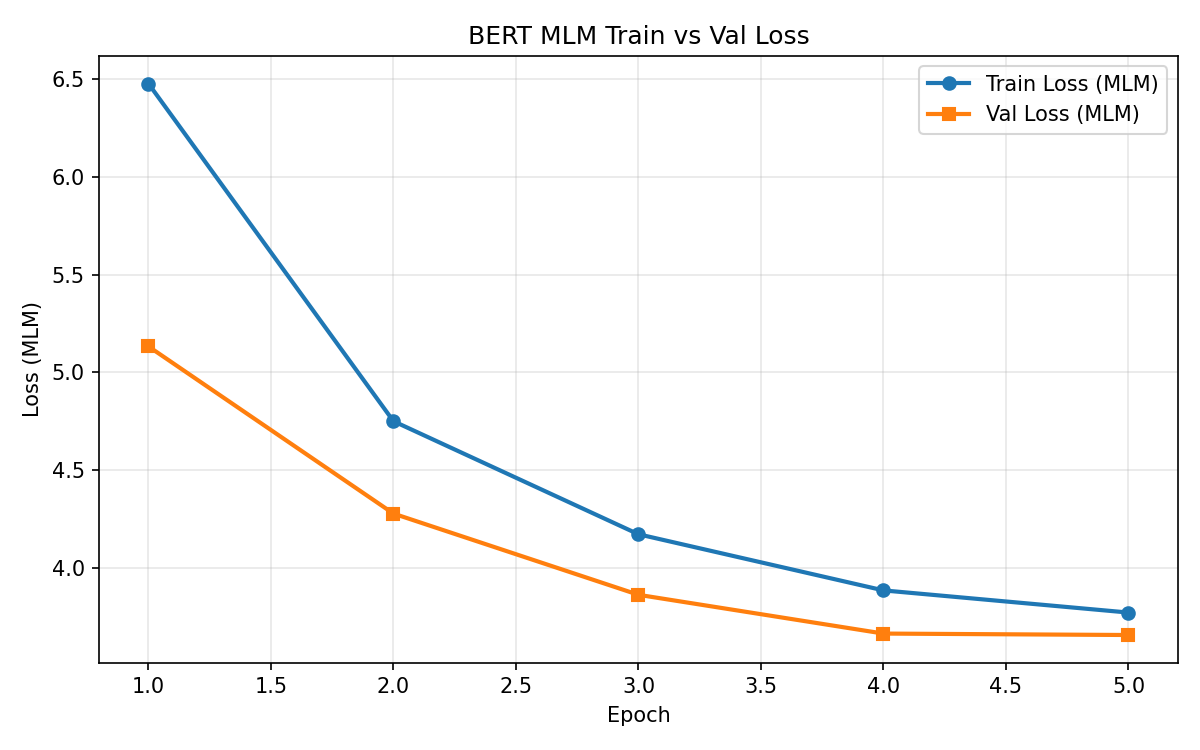
\includegraphics[width=\textwidth]{part2/outputs/bert_pretrain/loss_plot.png}
    \caption{Train and validation loss}
\end{subfigure}
\hfill
\begin{subfigure}[b]{0.48\textwidth}
    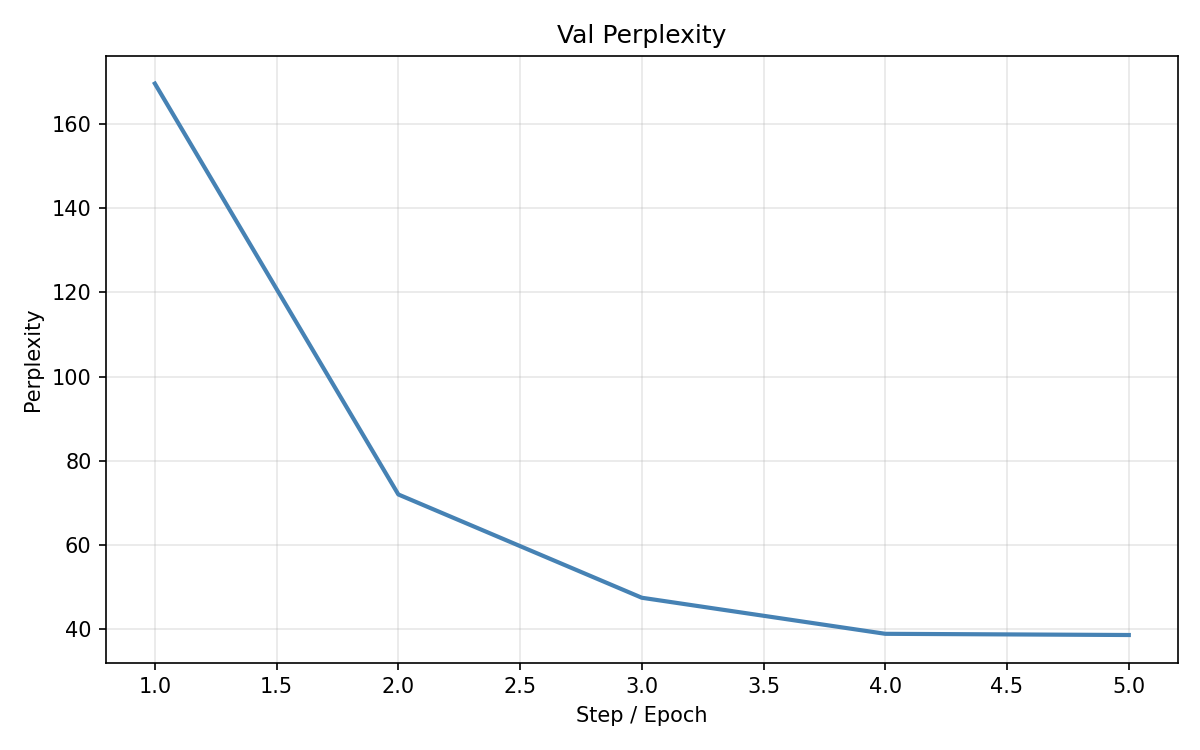
\includegraphics[width=\textwidth]{part2/outputs/bert_pretrain/val_ppl_plot.png}
    \caption{Validation perplexity}
\end{subfigure}

\vspace{0.5em}

\begin{subfigure}[b]{0.48\textwidth}
    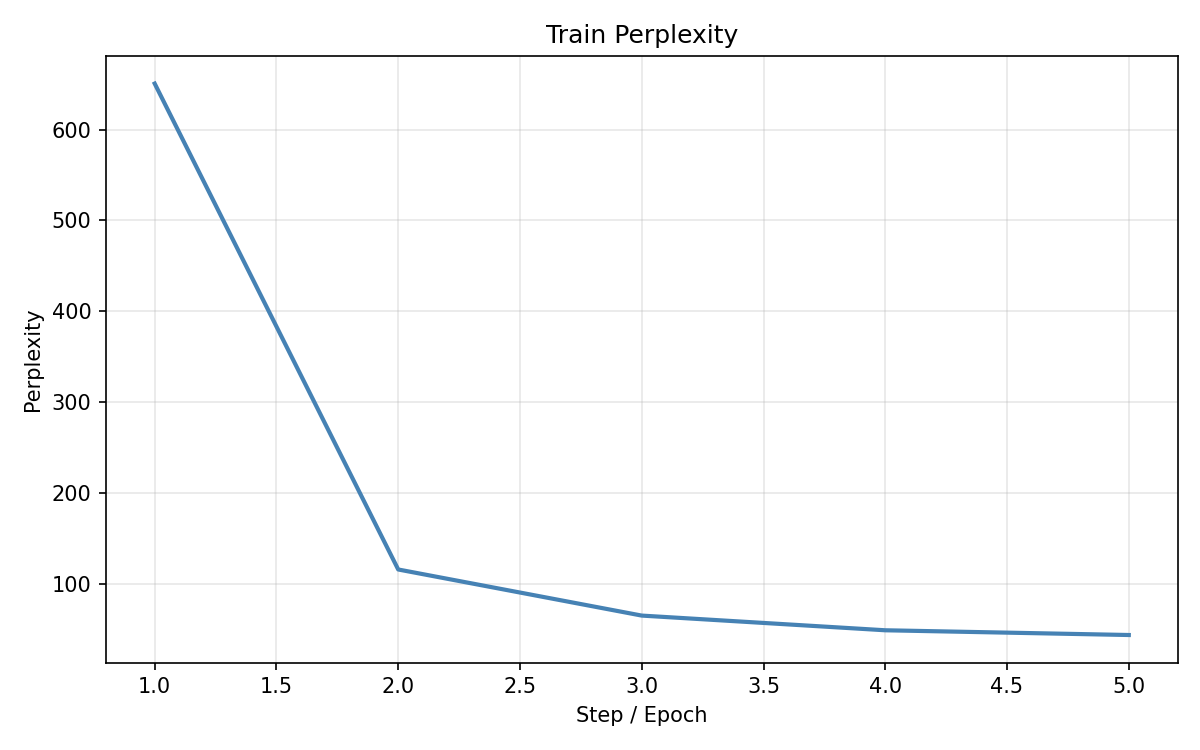
\includegraphics[width=\textwidth]{part2/outputs/bert_pretrain/train_ppl_plot.png}
    \caption{Training perplexity}
\end{subfigure}
\hfill
\begin{subfigure}[b]{0.48\textwidth}
    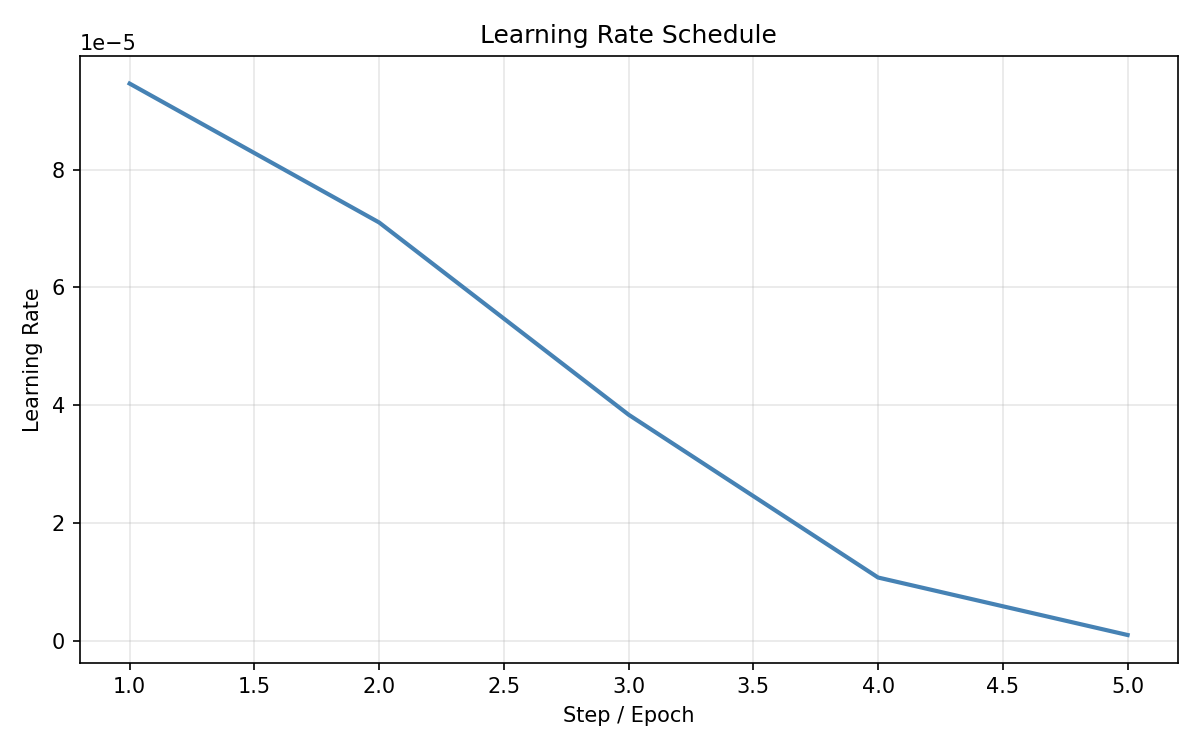
\includegraphics[width=\textwidth]{part2/outputs/bert_pretrain/lr_plot.png}
    \caption{Learning rate schedule}
\end{subfigure}
\caption{Part 2 — BERT pretraining curves over 5 epochs. Validation perplexity drops from 169.49 to 38.69.}
\label{fig:bert_pretrain}
\end{figure}

\subsubsection{GPT Pretraining}

\begin{table}[H]
\centering
\caption{GPT pretraining per-epoch results (5 epochs, 6.47 h)}
\label{tab:gpt_pretrain}
\begin{tabular}{ccccc}
\toprule
\textbf{Epoch} & \textbf{Train Loss} & \textbf{Val Loss} & \textbf{Train PPL} & \textbf{Val PPL} \\
\midrule
1 & 5.952 & 4.885 & 384.3 & 132.24 \\
2 & 4.628 & 4.316 & 102.4 & 74.85  \\
3 & 4.232 & 4.085 & 68.8  & 59.44  \\
4 & 4.042 & 3.988 & 56.9  & 53.93  \\
\textbf{5*} & \textbf{3.963} & \textbf{3.970} & \textbf{52.6} & \textbf{53.01} \\
\bottomrule
\multicolumn{5}{l}{\small * Best checkpoint (lowest val loss)}
\end{tabular}
\end{table}

\begin{figure}[H]
\centering
\begin{subfigure}[b]{0.48\textwidth}
    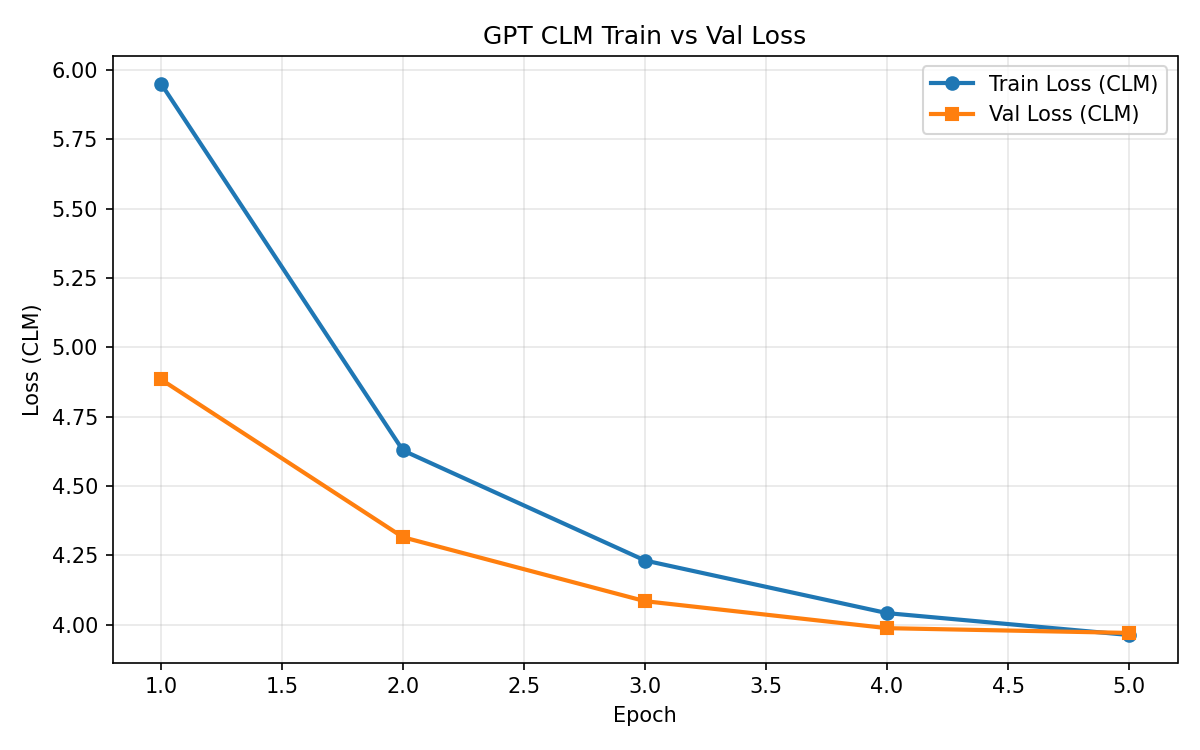
\includegraphics[width=\textwidth]{part2/outputs/gpt_pretrain/loss_plot.png}
    \caption{Train and validation loss}
\end{subfigure}
\hfill
\begin{subfigure}[b]{0.48\textwidth}
    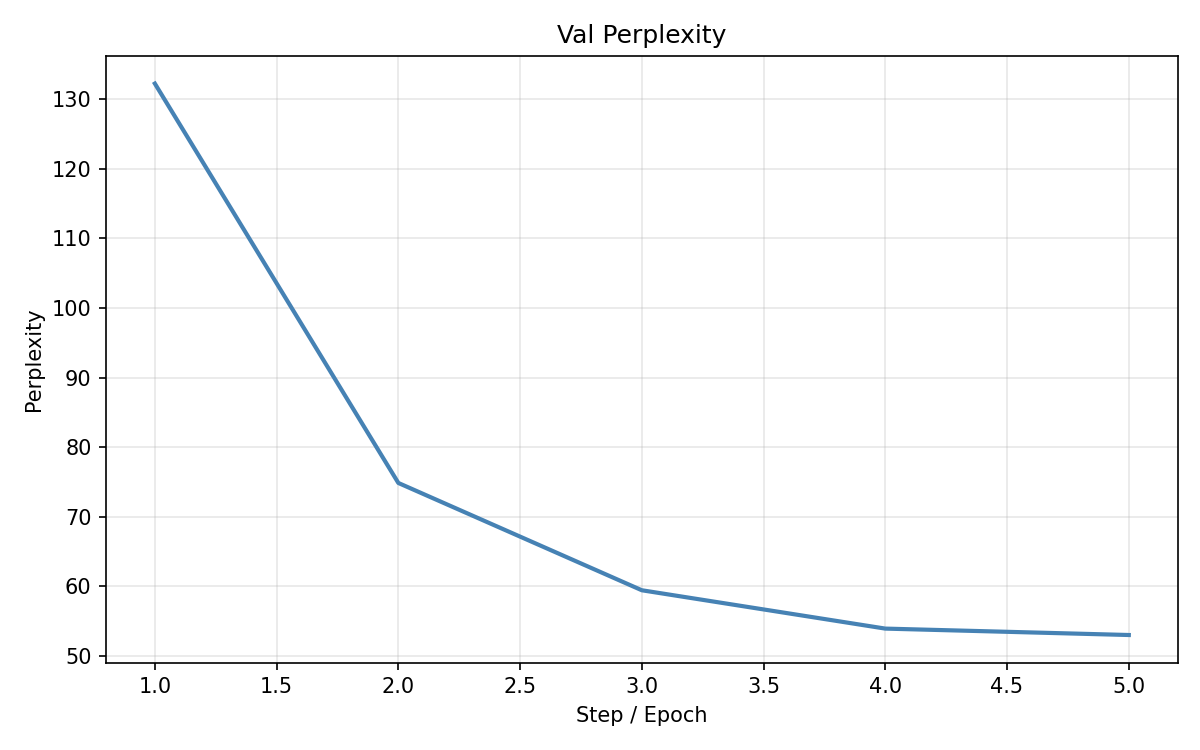
\includegraphics[width=\textwidth]{part2/outputs/gpt_pretrain/val_ppl_plot.png}
    \caption{Validation perplexity}
\end{subfigure}

\vspace{0.5em}

\begin{subfigure}[b]{0.48\textwidth}
    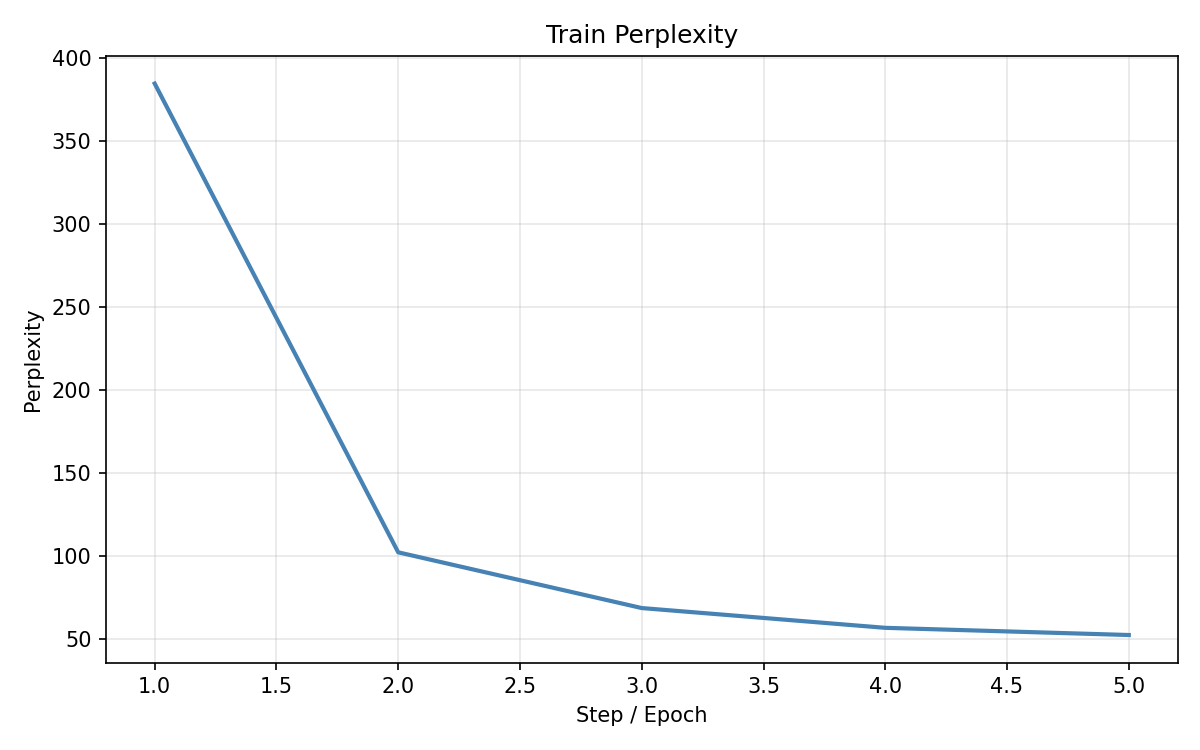
\includegraphics[width=\textwidth]{part2/outputs/gpt_pretrain/train_ppl_plot.png}
    \caption{Training perplexity}
\end{subfigure}
\hfill
\begin{subfigure}[b]{0.48\textwidth}
    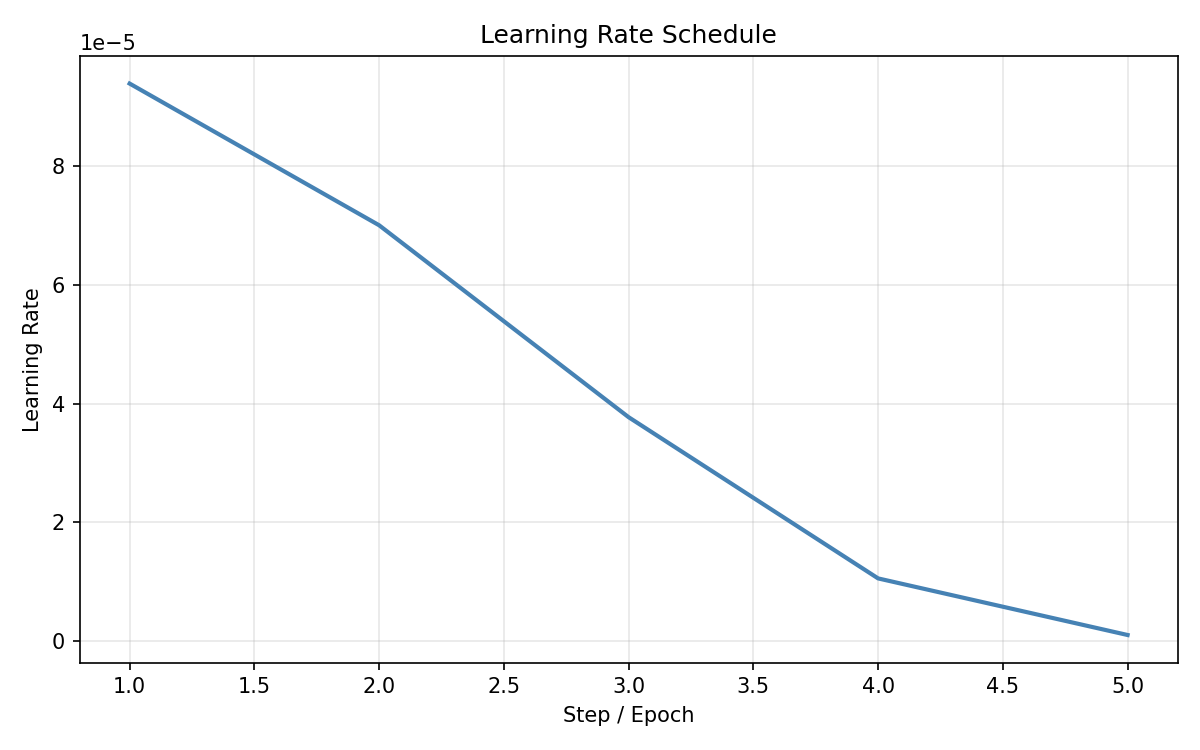
\includegraphics[width=\textwidth]{part2/outputs/gpt_pretrain/lr_plot.png}
    \caption{Learning rate schedule}
\end{subfigure}
\caption{Part 2 — GPT pretraining curves over 5 epochs. Validation perplexity drops from 132.24 to 53.01.}
\label{fig:gpt_pretrain}
\end{figure}

\subsubsection{Translation Fine-tuning}

\begin{table}[H]
\centering\small
\caption{Translation fine-tuning per-epoch results (5 epochs, 2.36 h)}
\label{tab:translation_finetune}
\begin{tabular}{ccccc}
\toprule
\textbf{Epoch} & \textbf{Train Loss} & \textbf{Val Loss} & \textbf{Val BLEU} & \textbf{Val CHRF++} \\
\midrule
\textbf{1*} & 2.210 & \textbf{0.036} & 27.85 & 60.40 \\
2 & 1.314 & 0.046 & 25.82 & 61.33 \\
3 & 1.307 & 0.052 & 31.33 & 68.58 \\
4 & 1.304 & 0.055 & 25.04 & 63.29 \\
5 & 1.303 & 0.056 & 25.70 & 63.24 \\
\bottomrule
\multicolumn{5}{l}{\small * Best checkpoint selected by lowest val loss}
\end{tabular}
\end{table}

\begin{figure}[H]
\centering
\begin{subfigure}[b]{0.48\textwidth}
    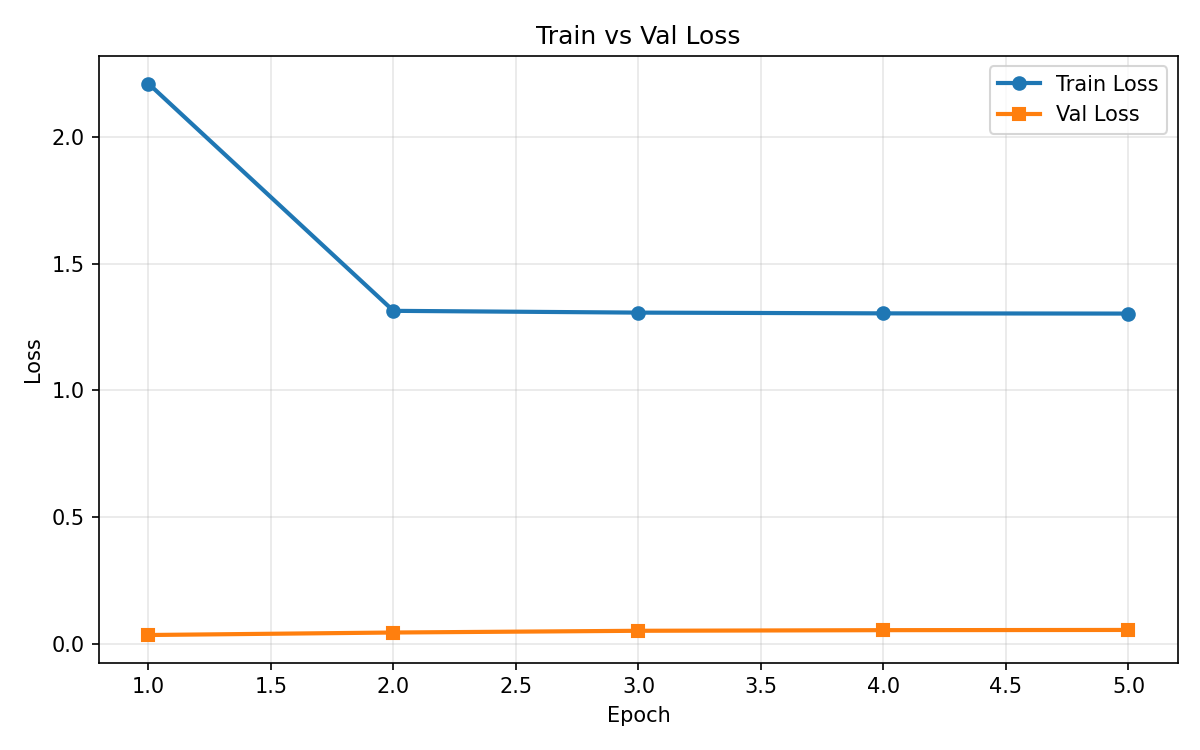
\includegraphics[width=\textwidth]{part2/outputs/translation/loss_plot.png}
    \caption{Train and validation loss}
\end{subfigure}
\hfill
\begin{subfigure}[b]{0.48\textwidth}
    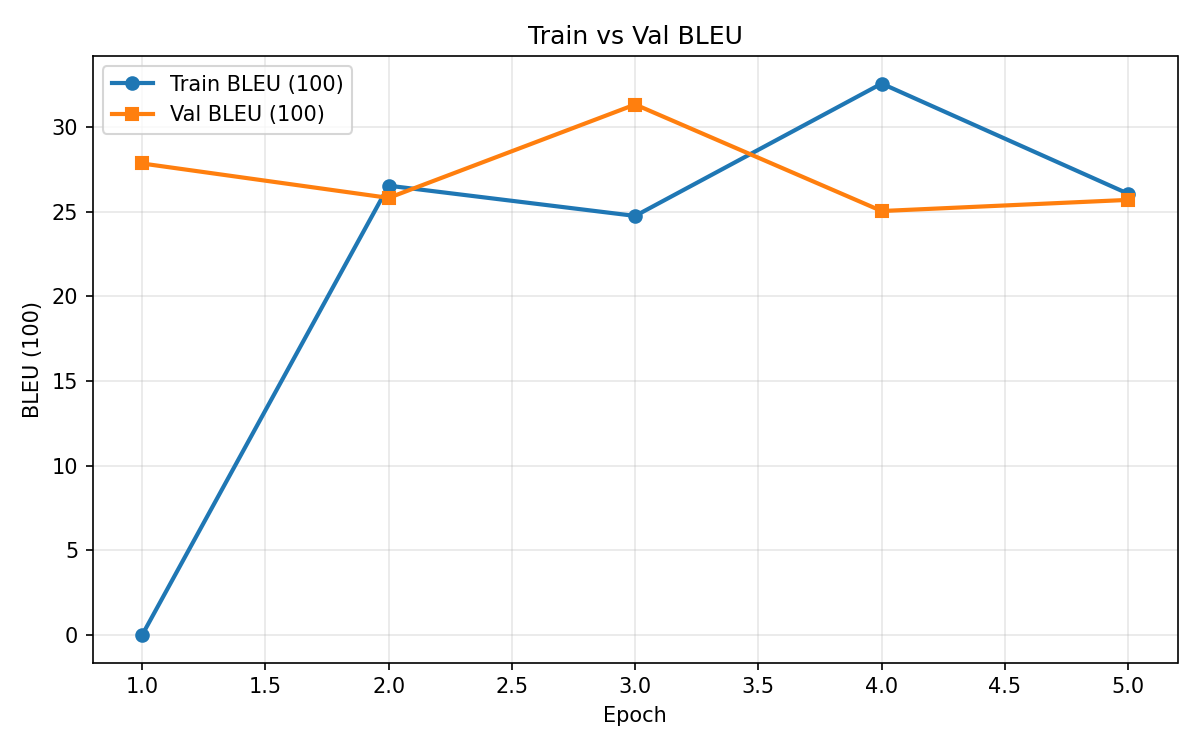
\includegraphics[width=\textwidth]{part2/outputs/translation/bleu_plot.png}
    \caption{Validation BLEU}
\end{subfigure}

\vspace{0.5em}

\begin{subfigure}[b]{0.48\textwidth}
    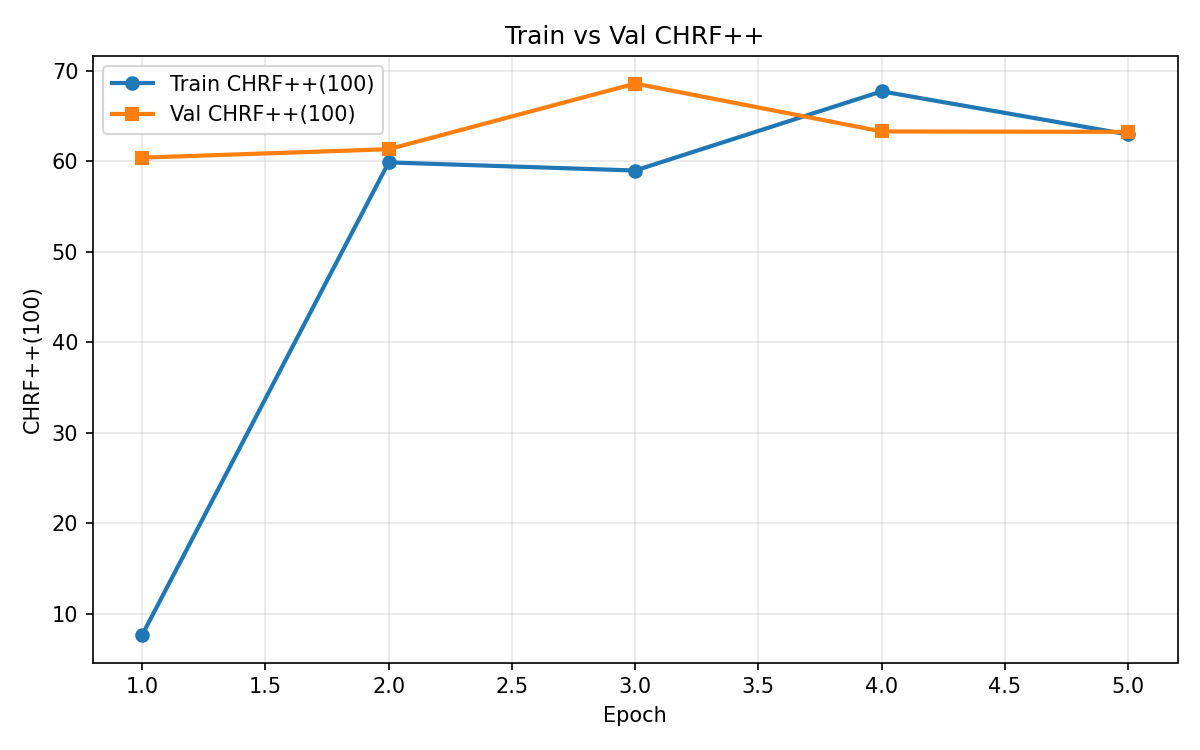
\includegraphics[width=\textwidth]{part2/outputs/translation/chrf_plot.png}
    \caption{Validation CHRF++}
\end{subfigure}
\hfill
\begin{subfigure}[b]{0.48\textwidth}
    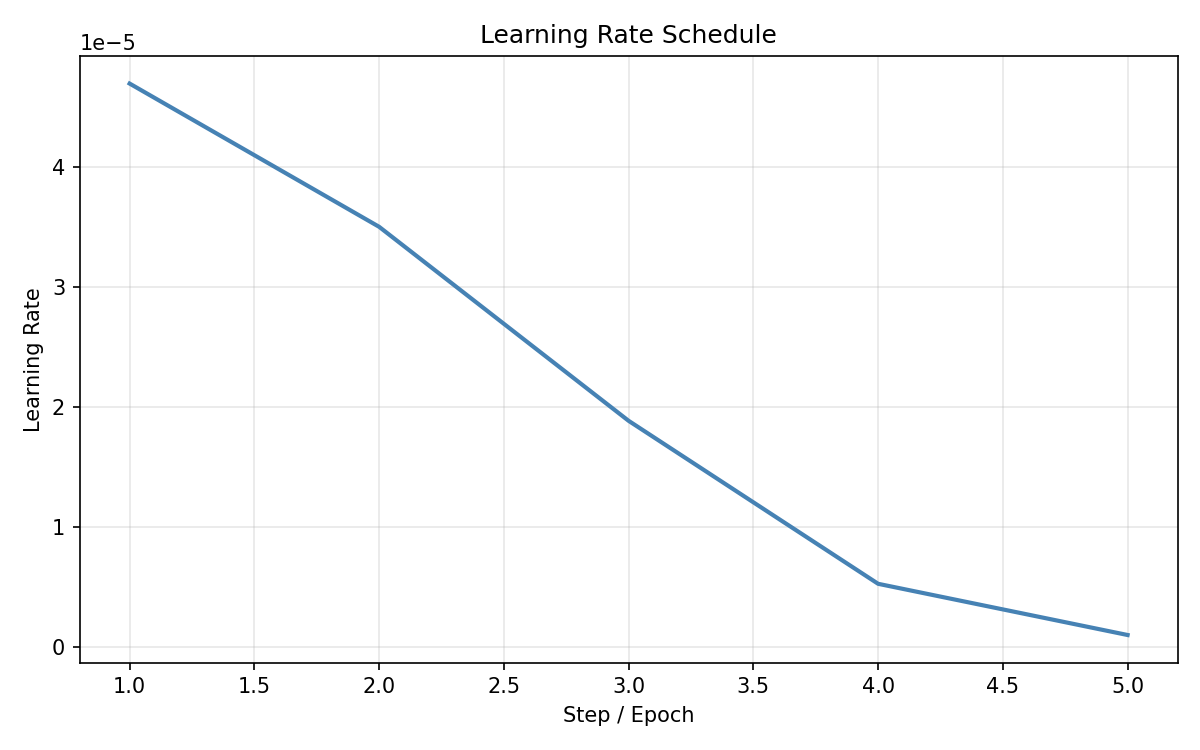
\includegraphics[width=\textwidth]{part2/outputs/translation/lr_plot.png}
    \caption{Learning rate schedule}
\end{subfigure}
\caption{Part 2 — Translation fine-tuning curves over 5 epochs. Best checkpoint (epoch 1) selected by lowest validation loss.}
\label{fig:translation_finetune}
\end{figure}

\subsubsection{Final Test Results}

\begin{table}[H]
\centering
\caption{Part 2 test set results (20,780 examples, greedy decoding)}
\label{tab:part2_results}
\begin{tabular}{ccc}
\toprule
\textbf{Test Loss} & \textbf{BLEU (100)} & \textbf{CHRF++ (100)} \\
\midrule
0.0383 & \textbf{25.46} & \textbf{57.71} \\
\bottomrule
\end{tabular}
\end{table}

\subsection{Analysis}

\subsubsection{Pretraining Effectiveness}

Both models show consistent and steady loss reduction across 5 epochs (Figures~\ref{fig:bert_pretrain} and~\ref{fig:gpt_pretrain}), validating the pretraining setup:
\begin{itemize}
    \item BERT val perplexity drops from 169.49 to 38.69 — a $4.4\times$ reduction, indicating the model learns meaningful contextual representations for Devanagari text.
    \item GPT val perplexity drops from 132.24 to 53.01 — a $2.5\times$ reduction, reflecting the harder causal LM objective.
    \item GPT achieves higher perplexity than BERT because CLM (predicting the next token given only left context) is inherently harder than MLM (predicting 15\% of tokens given full bidirectional context).
\end{itemize}

\subsubsection{Fine-tuning Dynamics}

An interesting observation is that the best checkpoint by validation loss is at epoch 1, despite later epochs showing higher validation BLEU scores (31.33 at epoch 3 vs 27.85 at epoch 1, see Figure~\ref{fig:translation_finetune}). This discrepancy arises because:
\begin{enumerate}
    \item The translation objective shifts from MLM/CLM log-likelihood to token-level cross-entropy with label smoothing, creating a different loss landscape.
    \item The cross-attention and LM head are randomly initialized: in epoch 1 the pretrained weights dominate and produce stable representations; later epochs show the model adapting further but with more variance.
    \item Val BLEU is noisy on the 48,400-example validation set with beam width 1.
\end{enumerate}

\subsubsection{Pretrained vs. From-Scratch}

The Part 2 model achieves BLEU = 25.46 compared to BLEU = 2.00 for the best Part 1 model — a \textbf{12.7$\times$ improvement}. This demonstrates the fundamental advantage of large-scale pretraining: the encoder-decoder system benefits from 11+ hours of language modeling on 504,474 monolingual sentences before seeing any parallel data, giving it strong Hindi and Marathi language priors that the LSTM must learn from scratch with only parallel supervision.

% ══════════════════════════════════════════════════════════════════════════════
\section{Overall Comparison}

\begin{table}[H]
\centering\small
\caption{Complete results comparison across all models and decoding strategies}
\label{tab:overall}
\begin{tabular}{llcc}
\toprule
\textbf{Part} & \textbf{Model} & \textbf{BLEU (100)} & \textbf{CHRF++ (100)} \\
\midrule
Part 1 & LSTM + Random embeddings (greedy) & 1.66 & 8.47 \\
Part 1 & LSTM + BERT embeddings (greedy)   & 0.97 & 7.96 \\
Part 1 & LSTM + Random embeddings (beam=2) & 2.00 & 9.34 \\
Part 1 & LSTM + BERT embeddings (beam=2)   & 1.98 & 9.46 \\
\midrule
\textbf{Part 2} & \textbf{BERT enc + GPT dec (greedy)} & \textbf{25.46} & \textbf{57.71} \\
\bottomrule
\end{tabular}
\end{table}

% ══════════════════════════════════════════════════════════════════════════════
\section{Failure Analysis and Limitations}

\subsection{Part 1}

\begin{itemize}
    \item \textbf{BERT embedding underperformance}: The vocabulary alignment between WordPiece and SentencePiece BPE via vector averaging is an approximation. A better approach would be to retrain the BERT model on the same SentencePiece vocabulary or fine-tune the BERT tokenizer.
    \item \textbf{Short training}: 10 epochs is insufficient for LSTM NMT convergence. Training curves (Figure~\ref{fig:random_training}) show no plateau — both models were still improving at epoch 10.
    \item \textbf{Teacher forcing gap}: The 50\% teacher forcing ratio during training differs significantly from the 0\% at evaluation, causing exposure bias.
\end{itemize}

\subsection{Part 2}

\begin{itemize}
    \item \textbf{Checkpoint selection inconsistency}: The best checkpoint at epoch 1 (by val loss) does not correspond to the best BLEU (epoch 3). A BLEU-based checkpoint selection strategy might yield higher test scores.
    \item \textbf{Short fine-tuning}: Only 5 fine-tuning epochs with a relatively small parallel corpus. More epochs and data augmentation could improve results.
    \item \textbf{Beam search timeout}: The beam=2 evaluation job did not complete within the allotted time, so only greedy results are reported for Part 2.
    \item \textbf{Pretraining scale}: 5 epochs on 504K sentences is modest. Models like BERT were pretrained on orders of magnitude more text.
\end{itemize}

% ══════════════════════════════════════════════════════════════════════════════
\section{Engineering Decisions}

\begin{itemize}
    \item \textbf{Shared SentencePiece vocabulary}: Exploits lexical overlap between Hindi and Marathi (both Devanagari script). Shared BPE subwords act as implicit cross-lingual anchors.
    \item \textbf{Bidirectional training with direction tokens}: A single model handles both translation directions, doubling the effective training data and encouraging the model to learn language-neutral representations.
    \item \textbf{Separate Part 2 tokenizer}: The \texttt{[MASK]} token required for MLM must occupy a fixed ID (4) determined before BPE training. This makes a new tokenizer necessary rather than patching the Part 1 tokenizer.
    \item \textbf{Gradient accumulation}: Effective batch sizes of 256 (BERT/GPT) and 128 (fine-tuning) are achieved via gradient accumulation without requiring multi-GPU training.
    \item \textbf{Label smoothing ($\varepsilon=0.1$)}: Applied in both experiments to prevent overconfident predictions and improve calibration.
\end{itemize}

% ══════════════════════════════════════════════════════════════════════════════
\section{LLM Usage Disclosure}

Claude (Anthropic) was used as a coding assistant throughout this project to accelerate development of boilerplate code, including training loop scaffolding, dataset classes, SLURM job scripts, and plotting utilities. All architectural decisions, hyperparameter choices, experimental design, and analysis presented in this report are the author's own work. All LLM-generated code was reviewed, understood, and modified before use. The author is prepared to independently explain and defend every aspect of both implementations.

% ══════════════════════════════════════════════════════════════════════════════
\section{Conclusion}

This work demonstrates the substantial gap between classical recurrent NMT and modern pretrained Transformer-based systems on Hindi$\leftrightarrow$Marathi translation. The LSTM + Bahdanau attention system provides a transparent, interpretable baseline (BLEU = 2.00 with beam search), while the pretrained BERT encoder + GPT decoder system achieves BLEU = 25.46 — a 12.7$\times$ improvement — primarily due to large-scale monolingual pretraining that provides strong language priors before parallel fine-tuning.

Key takeaways:
\begin{enumerate}
    \item Pretrained representations provide enormous value even when pretrained only on in-domain monolingual data (Hindi + Marathi), not multilingual corpora.
    \item The complementary nature of BERT (bidirectional context) and GPT (autoregressive generation) makes them naturally suited to the encoder and decoder roles in translation.
    \item Cross-attention, as the only randomly initialized component, is the bottleneck in the fine-tuning stage and would benefit most from additional training epochs.
    \item Classical LSTM systems remain informative baselines and are orders of magnitude cheaper to train and deploy.
\end{enumerate}

% ══════════════════════════════════════════════════════════════════════════════
\begin{thebibliography}{9}

\bibitem{bahdanau2015}
D. Bahdanau, K. Cho, and Y. Bengio,
\textit{Neural Machine Translation by Jointly Learning to Align and Translate},
International Conference on Learning Representations (ICLR), 2015.

\bibitem{vaswani2017}
A. Vaswani, N. Shazeer, N. Parmar, J. Uszkoreit, L. Jones, A. N. Gomez, L. Kaiser, and I. Polosukhin,
\textit{Attention Is All You Need},
Advances in Neural Information Processing Systems (NeurIPS), 2017.

\bibitem{devlin2019bert}
J. Devlin, M.-W. Chang, K. Lee, and K. Toutanova,
\textit{BERT: Pre-training of Deep Bidirectional Transformers for Language Understanding},
Annual Conference of the North American Chapter of the ACL (NAACL), 2019.

\bibitem{radford2019gpt2}
A. Radford, J. Wu, R. Child, D. Luan, D. Amodei, and I. Sutskever,
\textit{Language Models are Unsupervised Multitask Learners},
OpenAI Blog, 2019.

\bibitem{su2021roformer}
J. Su, Y. Lu, S. Pan, A. Murtadha, B. Wen, and Y. Liu,
\textit{RoFormer: Enhanced Transformer with Rotary Position Embedding},
arXiv preprint arXiv:2104.09864, 2021.

\bibitem{ainslie2023gqa}
J. Ainslie, J. Lee-Thorp, M. de Jong, Y. Zeiler, F. Lebron, and S. Sanghai,
\textit{GQA: Training Generalized Multi-Query Transformer Models from Multi-Head Checkpoints},
Empirical Methods in Natural Language Processing (EMNLP), 2023.

\bibitem{zhang2019rmsnorm}
B. Zhang and R. Sennrich,
\textit{Root Mean Square Layer Normalization},
Advances in Neural Information Processing Systems (NeurIPS), 2019.

\end{thebibliography}

\end{document}
